\chapter{Alberi}

{{[}CLRS{]} pp. 977-979}

\paragraph{{[}NO{]}Definizione}

{L'albero è un tipo particolare di grafo connesso, aciclico e non orientato.}

$G=(V,E)$ si dice albero {[}libero{]} se è aciclico e connesso.\\
Un albero libero in cui si seleziona un particolare vertice, chiamato ``radice'', si dice radicato.

{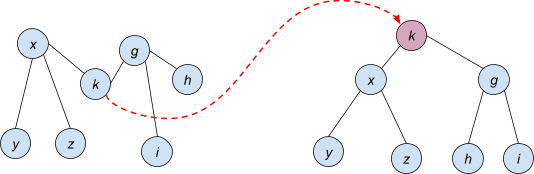
\includegraphics{images/image533.png}}

{Un albero radicato è una coppia $T=(N,A)$}

{$N$ è un insieme finito di nodi fra cui si distingue un nodo $R$, detto `Radice'.}

$A${~è un sottoinsieme del prodotto cartesiano $(NxN)$,è un insieme di coppie di nodi che chiamiamo archi.}

{In un albero, ogni nodo $v$ (eccetto la radice) ha esattamente un genitore che viene chiamato padre $u$, tale che $(u,v) \in A$}

\begin{figure}[H]
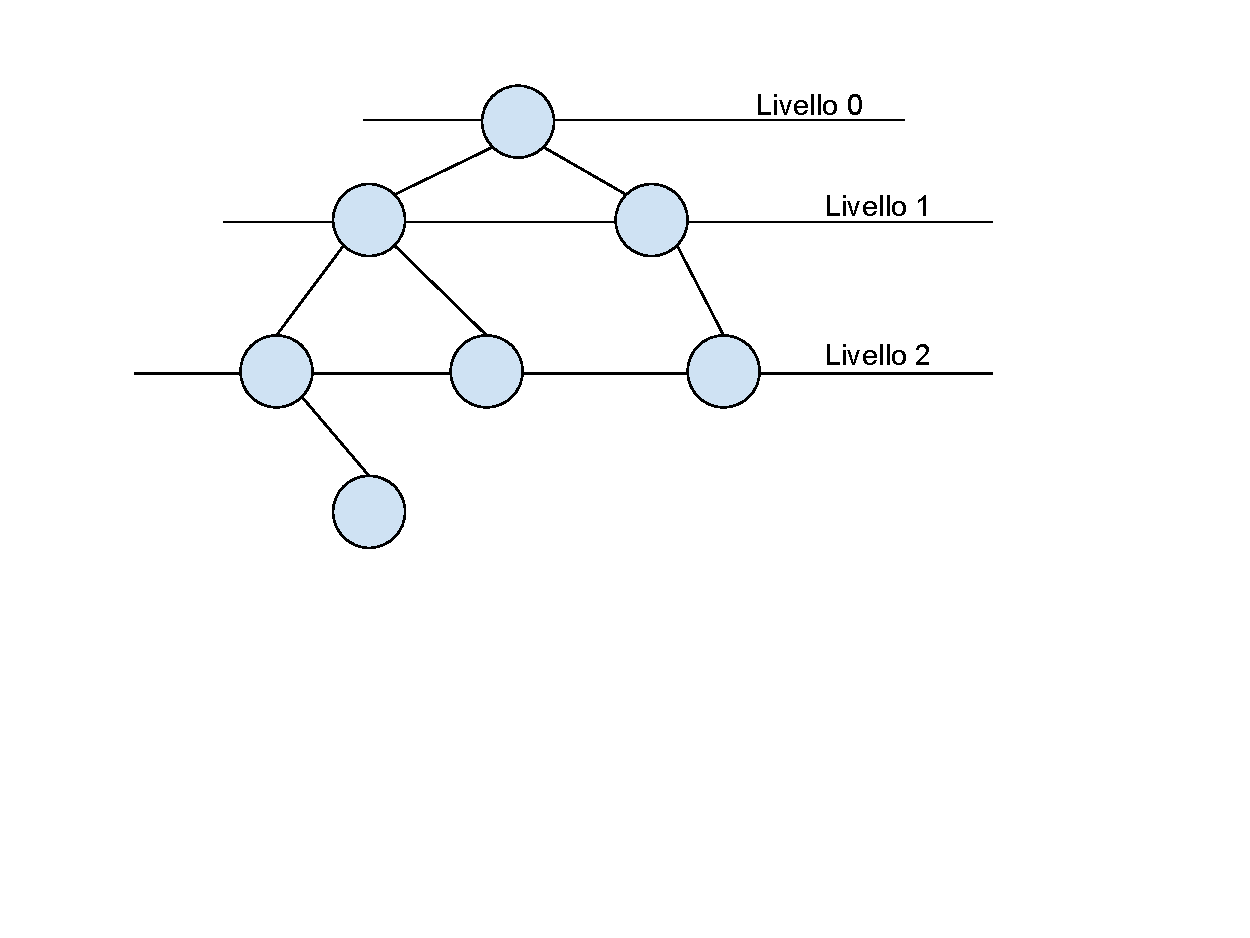
\includegraphics{graphs/alberi_livelli.pdf}
\end{figure}

{Un nodo può avere $0$ o più figli, un figlio è tale se esiste un arco $(u,v) \in A$}

{Il numero dei figli di un nodo si chiama GRADO del nodo.}

{Un nodo senza figli è detto FOGLIA o NODO ESTERNO.}

{Un nodo non foglia è un NODO INTERNO.}

{Se due nodi hanno lo stesso padre, allora sono fratelli.}

{Il cammino da $v$ a $v'$ nell'albero $T$ è una sequenza di nodi $n_0,n_1,\ldots,n_k$ tale che soddisfa queste condizioni:}

$v=n_0$

$v'=n_k$

$(n_{i-i},n_i) \in A\,\forall\,1>i>k$

{La lunghezza di un cammino è il numero di archi nel cammino oppure il numero di nodi diminuito di 1.}

{Sia $x$ un nodo dell'albero radicato $T$ con radice $r$.}

{Qualsiasi nodo $y$ in un cammino, che parte dalla radice $r$ ed arriva ad $x$, è detto ANTENATO di $x$($x$ compreso, è antenato di se stesso).}

{Se $y$ è un antenato di $x$, allora $x$ è DISCENDENTE di $y$}

{NB: Ogni nodo è DISCENDENTE ed ANTENATO di sè stesso.}

{Se $y$ è un antenato di $x$ ed $x$ è diverso da $y$, allora $y$ è un ANTENATO PROPRIO di $x$ ed $x$ è DISCENDENTE PROPRIO di $y$.}

{Il sottoalbero con radice in $x$ è l'albero indotto dai discendenti di $x$}

{La profondità di un nodo $x$ è la lunghezza del cammino dalla radice ad $x$.}

{Un livello di un albero è costituito da tutti i nodi che stanno alla stessa profondità. }

{L'altezza di un nodo $x$ è la lunghezza del più lungo cammino che scende da $x$ alle foglie (qualsiasi foglia) di profondità massima.}

{L'altezza di un albero è l'altezza del nodo radice.}

{L'altezza è la massima profondità di un qualsiasi nodo dell'albero.}

\section{Alberi binari}

{Gli alberi binari sono definiti in modo ricorsivo:}

\begin{itemize}
\tightlist
\item
  {Un albero vuoto è binario}
\item
  {Un albero costituito da un nodo (radice) ,}
\end{itemize}

{~~~~~~~~~~~~~~~~da un albero binario detto sottoalbero sinistro della
radice,}

{~~~~~~~~~~~~~~~~e da un'altro albero binario detto sottoalbero destro
della radice}

{~~~~~~~~~~~~~~~~è detto un albero binario.}

\subsection{Albero k-ario}

{E' un albero in cui i figli si un nodo sono etichettati con interi positivi distinti e le etichette maggiori di $K$ sono assenti = ogni nodo può avere al più $K$ figli.}

{Un albero K-ario completo è tale quando tutte le foglie hanno la stessa profondità e tutti i nodi interni hanno grado $K$}

\paragraph{Determinare la completezza}

{Trovare l'algoritmo per determinare la completezza di un albero}

{Dimostro per induzione che le foglie sono $K^h$}

{$h=0$ (caso base): $K^0=1$, OK}

{Assumiamo che per un albero di altezza $h$ sia vero che $n=K^h$}

{Lo dimostro per $h+1$}

{Il numero di nodi di profondità $h$ è $K^h$ per ipotesi}

{Il numero di nodi di profondità $h+1$ è $K^h*K=K^{h+1}$, OK}

\paragraph{Trovare il numero di foglie}

{Trovare il numero di foglie e il numero di nodi interni di un albero k-ario completo di altezza $h$}

{$\sum_{\varphi=0}^{h-1}{K^{\varphi}}$ è una sommatoria GEOMETRICA, si semplifica in $\frac{K^{h-1+1}-1}{K-1}$ con $k\neq 1$, quindi $\frac{K^h-1}{K-1}$}

{Altezza di un albero k-ario completo con $n$ nodi:}

$n=K^h \rightarrow log_k(n) = log_k(K^h) \rightarrow log_k(n) = h$

\paragraph{Proprietà}

{Dimostrare per induzione che in un albero BINARIO completo non nullo avente $n$ nodi, il numero di foglie è $\frac{n+1}{2}$}

\subsection{Tipo di dato ALBERO}

{Struttura:}

{Insieme di nodi}

{Insieme di archi}


\paragraph{Operazioni del tipo ALBERO}


{~~~~~~~~newTree() → T~~~~~~~~~~~~~~~~Nuovo albero T}

{~~~~~~~~numNodi(T) → int~~~~~~~~~~~~~~~~Numero di nodi presenti in T}

{~~~~~~~~grado(T,N) → int~~~~~~~~~~~~~~~~Numero di figli di N, N
appartenente a T}

{~~~~~~~~padre(T,N) → int~~~~~~~~~~~~~~~~Nodo padre, null se N è radice,
~N appartenente a T}

{~~~~~~~~figli(T,N) → int{[}{]}~~~~~~~~~~~~~~~~Lista contenente i figli
del nodo N, N appartenente a T}

{}

\section{Rappresentazione indicizzata di alberi}

\subsection{Utilizzo del vettore padri}

{Sia $T=(N,A), N = \{n_1,n_2,\ldots,n_n\}$}

{Costruisco un vettore di dimensione $n$, le cui celle contengono copie di $(i,u)$. Con $i$ indichiamo l'informazione del nodo e con $u$ indichiamo il nodo padre (indice).}

$\forall v \in [1,n]$

{p{[}v{]} → info = contenuto}

{p{[}v{]} → padre = indice del padre,$(u,v) \in A(archi)$, se $v$ è radice il padre è $NULL/-1/0$}

{Spazio per memorizzare $n=\Theta(n)$}

\paragraph{Implementazioni}

{Padre - Complessità $\Theta(1)$}

\lstinputlisting{code/tree_vecp_padre.txt}

{Figli - Complessità $\Theta(n)$}

\lstinputlisting{code/tree_vecp_figli.txt}

\subsection{Utilizzo del vettore posizionale}

{L'albero deve essere completo e con $k \geq 2$. La ricerca è ottimizzata rispetto all'albero dei padri. Ogni nodo ha una posizione prestabilita.}

{Utilizzo un vettore posizionale $P$ di dimensione $n$ tale che }

\begin{enumerate}
\tightlist
\item
  {0 è la posizione della radice}
\item
  {l'i-esimo figlio di un certo nodo $v$ è in posizione $kv+i+1$, con $0\leq i < K-1$}
\end{enumerate}

{un nodo $f$ è foglia se non ha figli, quindi se $kv+1>n$}

{Il padre del nodo $f$ è in posizione $\floor{\frac{f-1}{k}}$ (parte intera inferiore) e i figli si trovano tra $kv+1$ e $kv+1+i-1$.

\paragraph{Implementazioni}

{Padre - Complessità $\Theta(1)$}

\lstinputlisting{code/tree_vec_padre.txt}

{Figli - Complessità $\Theta(k)$, con $k$ = grado di $v$}

\lstinputlisting{code/tree_vec_figli.txt}

\section{Utilizzo di strutture collegate}

\subsection{Parent + Childs}

{Ogni nodo è un record con i seguenti campi:}

{~~~~~~~~k : informazione}

{~~~~~~~~p : puntatore al padre}

{~~~~~~~~Se il numero di figli è noto}

{~~~~~~~~~~~~~~~~left : puntatore al figlio sinistro}

{~~~~~~~~~~~~~~~~right : puntatore al figlio destro}

{Altrimenti si utilizza una lista di puntatori ai propri figli}

{$c[]$ : lista di puntatori ai figli~~~~~~~~}

{Se ogni nodo ha grado al più $k$, è possibile mantenere in ogni nodo un puntatore a ciascuno dei possibili $k$ figli}

{Spazio necessario: $\Theta(nk)$, se $k$ costante allora $\Theta(n)$}

\paragraph{Implementazioni:}

{Padre - Complessità $O(1)$}

\lstinputlisting{code/tree_pc_padre.txt}

{Figli - Complessità $O(k)$, con $k$ = grado di $v$ }

{Con $k$ non noto si utilizza un ciclo che scorre c{[}{]}}

\lstinputlisting{code/tree_pc_figli.txt}

\subsection{Parent + Left child + Right sibling}

{Ogni nodo è un record con i seguenti campi:}

{~~~~~~~~k : informazione}

{~~~~~~~~p : puntatore al padre}

{~~~~~~~~left\_child : puntatore al figlio sinistro}

{~~~~~~~~right\_sibling : puntatore al fratello immediatamente a destra}

\paragraph{Implementazioni}

{Padre - Complessità $\Theta(1)$}

\lstinputlisting{code/tree_plcrs_padre.txt}

{Figli - Complessità $\Theta(k)$ con $k$ = grado di $v$}

\lstinputlisting{code/tree_plcrs_figli.txt}

\section{Algoritmi di visita degli Alberi}

{{[}DFI{]} pp. 77-80}

\subsection{Visita generica}

\lstinputlisting{code/visita_generica.txt}

{Dimostrare che ha costo LINEARE}\textsuperscript{\protect\hyperlink{cmnt2}{{[}b{]}}}

\begin{teorema}{ }{theoexample}
L'algoritmo di visita, applicato alla radice di un albero con $m$ nodi, termina in $O(m)$ iterazioni. Lo spazio usato è $O(n)$
\end{teorema}

\paragraph{Dimostrazione}

{Hp: L'inserimento e la cancellazione da $S$ sono effettuati in tempo costante}

{Ogni nodo verrà inserito ed estratto dall'insieme $s$ una sola volta, perchè in un albero non si può tornare ad un nodo a partire dai suoi figli.}

{Quindi le iterazioni del ciclo while saranno al più $O(n)$}

{Poiché ogno nodo compare al più una volta in $S$, lo spazio richiesto non è più alto di $O(n)$}

\subsection{Visita DFS - Depth first search - Ricerca in profondità}

{Seguiamo tutti i figli sinistri, andando in profondità fino a che non si raggiunge la prima foglia sinistra. Solo quando il sottoalbero sx è stato completamente visitato, si passa ~a visitare il sottoalbero dx}

\lstinputlisting{code/dfs_visit.txt}

\subsection{Visita BFS - Breadth first search - Ricerca in ampiezza}

\paragraph{Proprietà 1}

Se $G$ è un albero, allora $\abs{E} = \abs{V} - 1$ poichè è, per definizione, connesso e aciclico:

\begin{itemize}
\tightlist
\item
  $G${~è connesso se $\abs{E} \geq \abs{V} - 1$ : si deve rispettare un numero minimo di archi}
\item
  $G${~è aciclico se $\abs{E} \leq \abs{V} - 1$ : si deve rispettare un numero massimo di archi}
\end{itemize}

{L'albero risulta essere quindi una struttura ``fragile'' per quanto riguarda il numero di archi.}

\paragraph{Proprietà degli alberi {[}liberi{]}}

{Sia $G=(V,E) [NO]$ , le seguenti affermazioni sono equivalenti:}

\begin{enumerate}
\tightlist
\item
  {$G$ è un albero}
\item
  {Due vertici qualsiasi di $G$ sono connessi da un unico cammino semplice, ovvero senza vertici ripetuti}
\end{enumerate}

\paragraph{Dimostrazione:}

{Sia $G=(V,E) [NO]$, per assurdo assumo ci siano almeno due vertici $u,v$, tali che esistono almeno due cammini che li collegano. Facendo ciò si forma un ciclo.}

\begin{enumerate}
\setcounter{enumi}{2}
\tightlist
\item
  $G${~è connesso, ma se un qualche
  arco viene rimosso da }$G${, il
  grafo risultante è disconnesso}
\item
  {$G$ è connesso e $\abs{E}=\abs{V}-1$}
\item
  {$G$ è aciclico e $\abs{E}=\abs{V}-1$}
\item
  {$G$ è aciclico, ma se un qualunque arco viene aggiunto, allora il grafo risultante è ciclico.}
\end{enumerate}

\section{Alberi di copertura}

{Un albero $G=(V,E) [NO]$ connesso si dice di copertura se tutti gli archi in $T \subseteq E$ toccano tutti i vertici di $G$.}

\subsection{Taglio di un albero}

{Un taglio di un albero è una divisione in due parti $(S,V\setminus S)$ dell'insieme dei vertici.}

{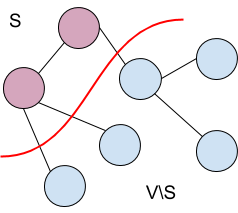
\includegraphics{images/image527.png}}

{Un taglio rispetta $A \subseteq E$ se non esistono archi di $A$ tagliati. Essi possono essere in una delle due partizioni ma non possono attraversare il taglio.}

\subsection{Arco leggero}

{Un arco è leggero se ha il peso minore tra gli altri archi attraversanti un taglio.}

